\chapter{Experiments\label{chap:experiments}}

This chapter discusses the initial experiments conducted on the dataset and their results.

\begin{figure}[htb]
	\centering
	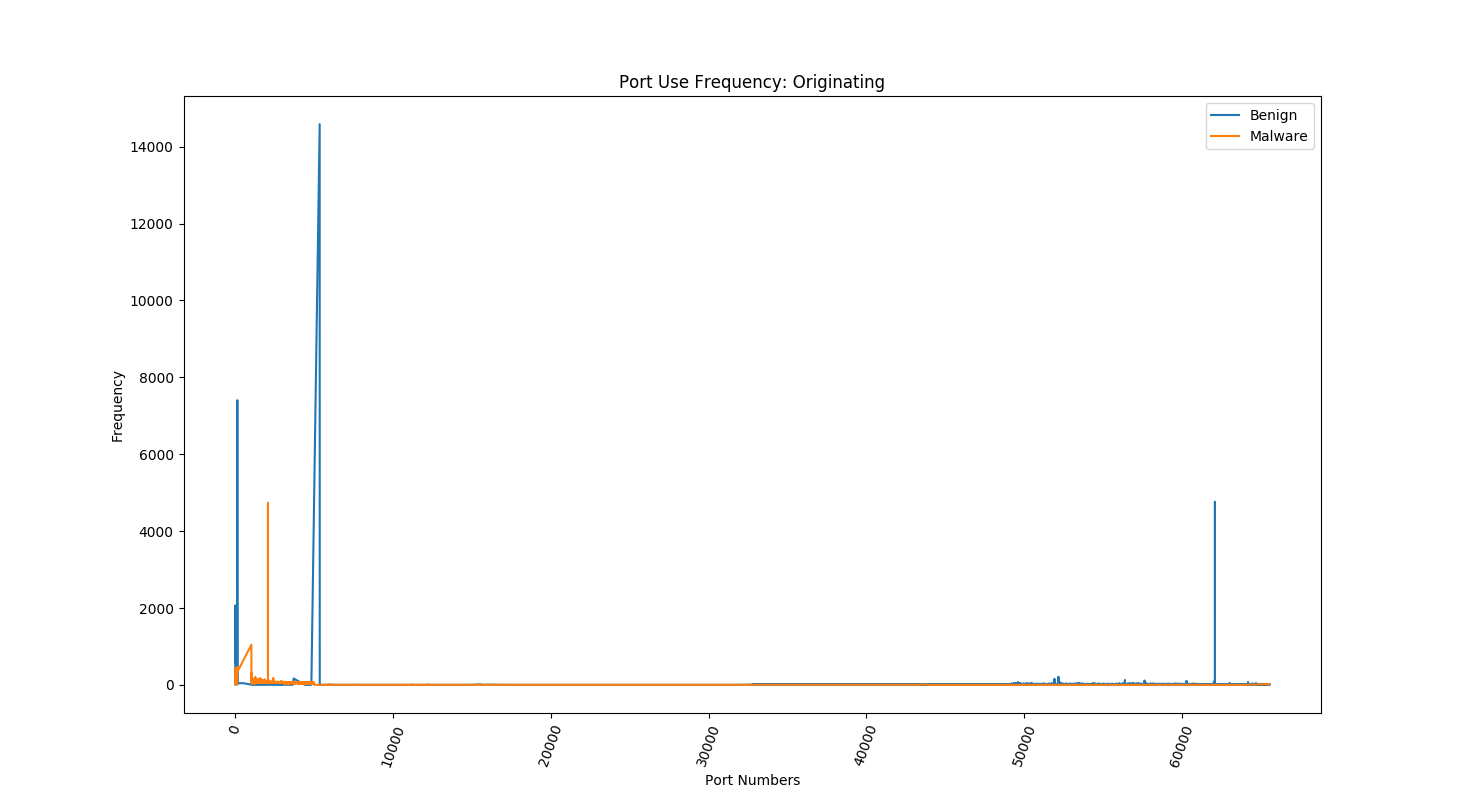
\includegraphics[width=1\textwidth]{images/orig-port-freq.png}
	\caption{Frequency of ports used by ORIG} 
	\label{fig:orig-port-freq}
\end{figure}

\begin{figure}[htb]
	\centering
	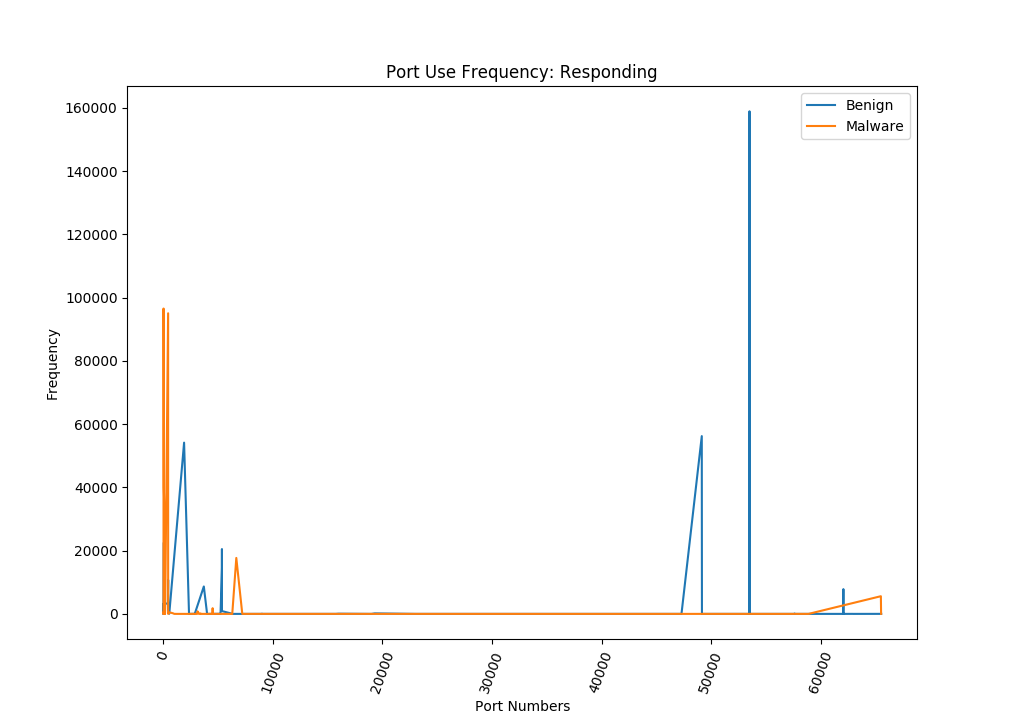
\includegraphics[width=1\textwidth]{images/resp-port-freq.png}
	\caption{Frequency of ports used by RESP} 
	\label{fig:resp-port-freq}
\end{figure}

As we can see from Figure \ref{fig:orig-port-freq}, the most frequent ports in malware captures are different than the most frequent ports in benign captures. We can see a similar result in Figure \ref{fig:resp-port-freq} where we plot the frequency of ports used by the responding endpoint in the network traffic capture. The top 5 ports with most frequency in both the captures are shown in Table \ref{tab:3}.

\begin{table}[!htb]
	\caption{Top Five Ports Used by ORIG\label{tab:3}}
	\begin{center}
		\begin{tabular}{c|p{0.15\textwidth}|p{0.50\textwidth}}\hline\hline
			Dataset & Port Number & \multicolumn{1}{l}{Known Port Assignments} \\ \hline
			Malware & 2077 & WebDisk or Old Tivoli Storage \\
			& 2079	&  IDWARE Router Port\\
			& 1025	&  Ports > 1024 are designated for dynamic allocation by Windows\\
			& 137	&  File and Print Sharing under Windows\\
			& 3 &  Compression Process \\ \hline
			Benign & 5353  &  Multicast DNS, iChat, Mac OS X Bonjour\\
			& 135 &  Remote Procedure Call (RPC)\\
			& 62078 &  UPnP (Universal Plug and Play), iTunes\\
			& 137 &  File and Print Sharing under Windows\\
			& 138 &  File and Print Sharing under Windows\\
			\hline\hline
		\end{tabular}
	\end{center}
\end{table}

\begin{table}[!htb]
	\caption{Top Five Ports Used by RESP\label{tab:4}}
	\begin{center}
		\begin{tabular}{c|p{0.15\textwidth}|p{0.50\textwidth}}\hline\hline
			Dataset & Port Number & \multicolumn{1}{l}{Known Port Assignments} \\ \hline
			Malware & 25 & SMTP (Simple Mail Transfer Protocol) \\
			& 443	&  HTTPS / SSL - encrypted web traffic\\
			& 53	&  DNS (Domain Name Service)\\
			& 80	&  Hyper Text Transfer Protocol (HTTP) \\
			& 6667 &  IRC (Internet Relay Chat) \\ \hline
			Benign & 53508  &  Xsan Filesystem Apple\\
			& 49153 &  ANTLR, ANother Tool for Language Recognition\\
			& 1900 &  IANA registered by Microsoft for SSDP (Simple Service Discovery Protocol)\\
			& 53 &  DNS (Domain Name Service)\\
			& 5355 &  Link-Local Multicast Name Resolution Windows\\
			\hline\hline
		\end{tabular}
	\end{center}
\end{table}

As we can see from Table \ref{tab:3} and Table \ref{tab:4}, malware dataset had Internet Relay Chat (IRC) port among the most frequently used. We know that most of the malware use IRC to exfiltrate data from the infected system to other systems. We also see that HTTPS port 443 is also among the most frequently used in the malware captures.

\section{K-means Clustering}

K-means clustering is an unsupervised learning algorithm that aims to partition \verb|n| data points into \verb|k| clusters. Clustering is used to see whether the data points naturally form distinct clusters or whether they are similar to other data points in the dataset. We normalized the values in our dataset and performed K-means clustering with \verb|k=2|. The results are shown in the following figures:

\begin{figure}[htb]
	\centering
	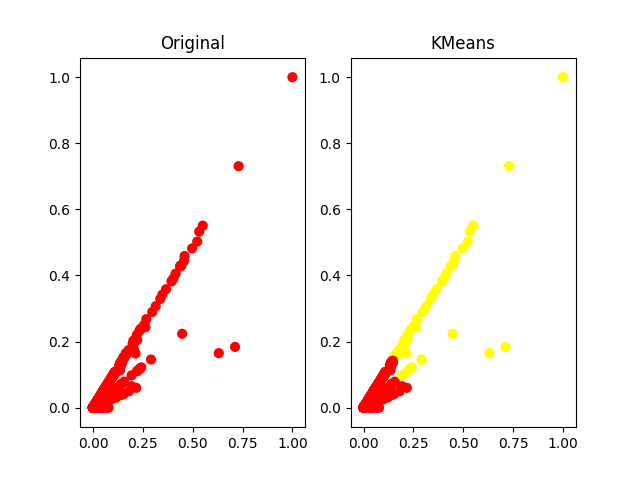
\includegraphics[width=1\textwidth]{images/kmeans.png}
	\caption{Original Scatter Plot vs K-means clustering} 
	\label{fig:kmeans1}
	
	\centering
	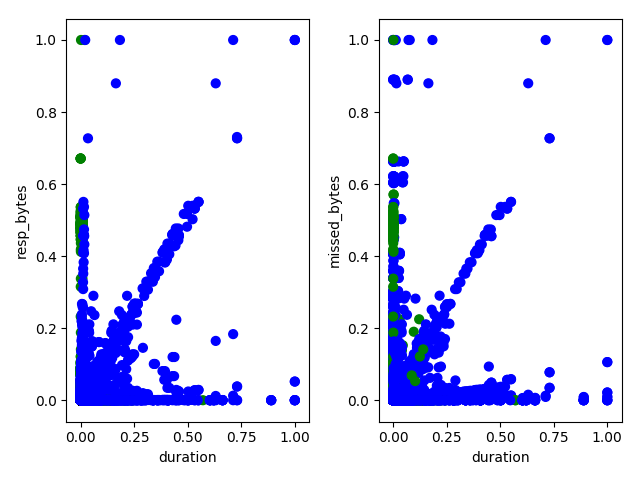
\includegraphics[width=1\textwidth]{images/kmeans2.png}
	\caption{Original Scatter Plots with different axes} 
	\label{fig:kmeans2}
\end{figure}

As seen in Figure \ref{fig:kmeans1}, K-means didn't really give us distinct clusters. Also , the most of the scatter plots based on connection features resemble that in Figure \ref{fig:kmeans2}. We can further perform experiments such as Support Vector Machine (SVM) and Principal Component Analysis (PCA) to find prominent features in the dataset.